\documentclass[9pt,letter]{article}
\usepackage{lmodern}
\usepackage{amssymb,amsmath}
\usepackage{ifxetex,ifluatex}
\usepackage{fixltx2e} % provides \textsubscript
\ifnum 0\ifxetex 1\fi\ifluatex 1\fi=0 % if pdftex
  \usepackage[T1]{fontenc}
  \usepackage[utf8]{inputenc}
\else % if luatex or xelatex
  \ifxetex
    \usepackage{mathspec}
  \else
    \usepackage{fontspec}
  \fi
  \defaultfontfeatures{Ligatures=TeX,Scale=MatchLowercase}
\fi
% use upquote if available, for straight quotes in verbatim environments
\IfFileExists{upquote.sty}{\usepackage{upquote}}{}
% use microtype if available
\IfFileExists{microtype.sty}{%
\usepackage{microtype}
\UseMicrotypeSet[protrusion]{basicmath} % disable protrusion for tt fonts
}{}
\usepackage[margin=.75in]{geometry}
\usepackage{hyperref}
\hypersetup{unicode=true,
            pdftitle={Assignment 3},
            pdfauthor={Azoacha Forcheh, 20558994},
            pdfborder={0 0 0},
            breaklinks=true}
\urlstyle{same}  % don't use monospace font for urls
\usepackage{color}
\usepackage{fancyvrb}
\newcommand{\VerbBar}{|}
\newcommand{\VERB}{\Verb[commandchars=\\\{\}]}
\DefineVerbatimEnvironment{Highlighting}{Verbatim}{commandchars=\\\{\}}
% Add ',fontsize=\small' for more characters per line
\usepackage{framed}
\definecolor{shadecolor}{RGB}{248,248,248}
\newenvironment{Shaded}{\begin{snugshade}}{\end{snugshade}}
\newcommand{\KeywordTok}[1]{\textcolor[rgb]{0.13,0.29,0.53}{\textbf{#1}}}
\newcommand{\DataTypeTok}[1]{\textcolor[rgb]{0.13,0.29,0.53}{#1}}
\newcommand{\DecValTok}[1]{\textcolor[rgb]{0.00,0.00,0.81}{#1}}
\newcommand{\BaseNTok}[1]{\textcolor[rgb]{0.00,0.00,0.81}{#1}}
\newcommand{\FloatTok}[1]{\textcolor[rgb]{0.00,0.00,0.81}{#1}}
\newcommand{\ConstantTok}[1]{\textcolor[rgb]{0.00,0.00,0.00}{#1}}
\newcommand{\CharTok}[1]{\textcolor[rgb]{0.31,0.60,0.02}{#1}}
\newcommand{\SpecialCharTok}[1]{\textcolor[rgb]{0.00,0.00,0.00}{#1}}
\newcommand{\StringTok}[1]{\textcolor[rgb]{0.31,0.60,0.02}{#1}}
\newcommand{\VerbatimStringTok}[1]{\textcolor[rgb]{0.31,0.60,0.02}{#1}}
\newcommand{\SpecialStringTok}[1]{\textcolor[rgb]{0.31,0.60,0.02}{#1}}
\newcommand{\ImportTok}[1]{#1}
\newcommand{\CommentTok}[1]{\textcolor[rgb]{0.56,0.35,0.01}{\textit{#1}}}
\newcommand{\DocumentationTok}[1]{\textcolor[rgb]{0.56,0.35,0.01}{\textbf{\textit{#1}}}}
\newcommand{\AnnotationTok}[1]{\textcolor[rgb]{0.56,0.35,0.01}{\textbf{\textit{#1}}}}
\newcommand{\CommentVarTok}[1]{\textcolor[rgb]{0.56,0.35,0.01}{\textbf{\textit{#1}}}}
\newcommand{\OtherTok}[1]{\textcolor[rgb]{0.56,0.35,0.01}{#1}}
\newcommand{\FunctionTok}[1]{\textcolor[rgb]{0.00,0.00,0.00}{#1}}
\newcommand{\VariableTok}[1]{\textcolor[rgb]{0.00,0.00,0.00}{#1}}
\newcommand{\ControlFlowTok}[1]{\textcolor[rgb]{0.13,0.29,0.53}{\textbf{#1}}}
\newcommand{\OperatorTok}[1]{\textcolor[rgb]{0.81,0.36,0.00}{\textbf{#1}}}
\newcommand{\BuiltInTok}[1]{#1}
\newcommand{\ExtensionTok}[1]{#1}
\newcommand{\PreprocessorTok}[1]{\textcolor[rgb]{0.56,0.35,0.01}{\textit{#1}}}
\newcommand{\AttributeTok}[1]{\textcolor[rgb]{0.77,0.63,0.00}{#1}}
\newcommand{\RegionMarkerTok}[1]{#1}
\newcommand{\InformationTok}[1]{\textcolor[rgb]{0.56,0.35,0.01}{\textbf{\textit{#1}}}}
\newcommand{\WarningTok}[1]{\textcolor[rgb]{0.56,0.35,0.01}{\textbf{\textit{#1}}}}
\newcommand{\AlertTok}[1]{\textcolor[rgb]{0.94,0.16,0.16}{#1}}
\newcommand{\ErrorTok}[1]{\textcolor[rgb]{0.64,0.00,0.00}{\textbf{#1}}}
\newcommand{\NormalTok}[1]{#1}
\usepackage{graphicx,grffile}
\makeatletter
\def\maxwidth{\ifdim\Gin@nat@width>\linewidth\linewidth\else\Gin@nat@width\fi}
\def\maxheight{\ifdim\Gin@nat@height>\textheight\textheight\else\Gin@nat@height\fi}
\makeatother
% Scale images if necessary, so that they will not overflow the page
% margins by default, and it is still possible to overwrite the defaults
% using explicit options in \includegraphics[width, height, ...]{}
\setkeys{Gin}{width=\maxwidth,height=\maxheight,keepaspectratio}
\IfFileExists{parskip.sty}{%
\usepackage{parskip}
}{% else
\setlength{\parindent}{0pt}
\setlength{\parskip}{6pt plus 2pt minus 1pt}
}
\setlength{\emergencystretch}{3em}  % prevent overfull lines
\providecommand{\tightlist}{%
  \setlength{\itemsep}{0pt}\setlength{\parskip}{0pt}}
\setcounter{secnumdepth}{0}
% Redefines (sub)paragraphs to behave more like sections
\ifx\paragraph\undefined\else
\let\oldparagraph\paragraph
\renewcommand{\paragraph}[1]{\oldparagraph{#1}\mbox{}}
\fi
\ifx\subparagraph\undefined\else
\let\oldsubparagraph\subparagraph
\renewcommand{\subparagraph}[1]{\oldsubparagraph{#1}\mbox{}}
\fi

%%% Use protect on footnotes to avoid problems with footnotes in titles
\let\rmarkdownfootnote\footnote%
\def\footnote{\protect\rmarkdownfootnote}

%%% Change title format to be more compact
\usepackage{titling}

% Create subtitle command for use in maketitle
\newcommand{\subtitle}[1]{
  \posttitle{
    \begin{center}\large#1\end{center}
    }
}

\setlength{\droptitle}{-2em}
  \title{Assignment 3}
  \pretitle{\vspace{\droptitle}\centering\huge}
  \posttitle{\par}
\subtitle{STAT 442: Data Visualization}
  \author{Azoacha Forcheh, 20558994}
  \preauthor{\centering\large\emph}
  \postauthor{\par}
  \date{}
  \predate{}\postdate{}

\usepackage{graphicx}
\usepackage{color}
\usepackage{enumitem}
\newcommand{\benum}{\begin{enumerate}}
\newcommand{\eenum}{\end{enumerate}}
\newcommand{\bitem}{\begin{itemize}}
\newcommand{\eitem}{\end{itemize}}

\begin{document}
\maketitle

\benum
\item \textbf{Stem and leaf plots.}

\benum
\item \textbf{(3 marks)} What characteristics of the data can you see
(or easily determine) from the stem and leaf display? DO NOT hand these
displays in!

\bitem
\item Plot 1: The density of the data seems to take on the shape of a
somewhat flat bell curve centred at around \(-0.4 - 0\), with very
little spread. It appears to be trimodal, with all the modes appearing
between -1 and 1. \item Plot 2: The density of the data seems to take on
the shape of a steep bell curve centred at around \(-0.4 - 0\), with an
average amount of spread. It appears to be unimodal at around
\(-0.4 - 0\). \item Plot 3: The density of the data seems to take on the
shape of the bell curve of a standard normal distribution, centred at
around \(-0.4 - 0\), with somewhat even spread on either side of the
peak. It appears to be unimodal at around \(-0.4 - 0\). In addition, the
value of \(-3.4\) seems to be an outlier. \item Plot 4: The density of
the data seems to take on the shape of a very steep bell curve, centred
at around \(0 - 0.4\), with very little spread and very short tails. It
appears to be unimodal at around \(-0.4 - 0\). In addition, the value of
\(-3.4\) seems to be an outlier. \item Plot 5: The data appears to be
bimodal, with the modes at around \(-0.3 - -0.2\) and \(0.2 - 0.3\). In
addition, the values of \(-3.1, -3.0\) seems to be an outlier. \eitem

\item 

\textbf{(2 marks)} How does the stem and leaf adapt to increasing sample
size? How would the stem and leaf display have to be displayed for a
sample of \(n=10,000\) and what would be the problems, if any, with
that?

The scale of the plot decreases as n increases. With these plots, the
number of parts of each stem was reduced from 5 (i.e.~the possible
digits of the leaves were split into 2 groups of 5) for
\(n \in\ \{30, 100, 200\}\) to 2 for \(n \in\ \{500, 1000\}\) (i.e.~the
possible digits of the leaves were split into 5 groups of 2).

In addition, for the stems not containing 8 and 9, the label for the
stems change from the value of the digit for (e.g. \(-1.\)) to the first
letter of the digits of the group (`t' for 2 and 3, `f' for 4 and 5, `s'
for 6 and 7).

According to the documentation for \textbf{stem.leaf}, the possible
number of parts that the stem can be separated into is one of 1, 2, or
5. So for \(n=10,000\), each time will be separated into 5 groups of 2
digits. As a result, the stems of the plot will be extremely long as
\(n\) is extremely high. This will make it easier to determine the
general pattern of the data as it will be spread more horizontally
instead of vertically, making the shape of the density clearer. However,
the tradeoff is that the detailed pattern becomes much harder to
interpret due to the high number of data points and the comparatively
small number of parts in each stem. \eenum

\item 

\textbf{Quantile functions.} Suppose a continuous random variate \(X\)
has a strictly increasing cumulative distribution function \(F_X(x)\), a
continuous density \(f_X(x)\), and a quantile function \(Q_X(p)\).

\benum
\item \textbf{(2 marks)} Suppose \(U \sim U(0,1)\). Define a random
variate \(Y=Q_X(U)\). Prove that \(Pr(Y \le a) = F_X(a)\) for any value
of \(a\), and hence that \(Y\) has the same distribution as does \(X\).

Note that \(F_X(x)\) is continuous and strictly increasing. Hence,
\(Q_X(x) = F_X^{-1}(x) \implies F_X(x) = Q_X^{-1}(x)\). So: \[
\begin{array}{rcll}
Pr(Y \le a) &=& Pr(Q_X(U) \le a)\\
&=& Pr(U \le Q_X^{-1}(a))\\
&=& Q_X^{-1}(a) & \text{since } U \sim U(0,1)\\
&=& F_X(a)\\
\end{array}
\]

\item 

\textbf{(4 marks)} Let \(Y = aX +b\) for some constants \(a > 0\) and
\(b\). Prove that the quantile function \(Q_Y(p)\) for \(Y\) is related
to that of \(X\) as \[ Q_Y(p) = a Q_X(p) + b. \]

First, note that since \(F_X(x)\) is a strictly increasing c.d.f and
\(Y = aX +b\) for some constants \(a > 0\) (so \(Y\) increases as \(X\)
increases) and \(b\), \(F_Y(y)\) is also a continuous, strictly
continuous c.d.f. We use this to prove the given statement as follows:

\[
\begin{array}{rcll}
Pr(X \le Q_X(p)) &=& F_X(Q_X(p))\\
&=& F_X(F^{-1}_X(p)) & \text{since } F_X \text{ is continous and strictly increasing}\\
&=& p\\
p &=& Pr(X \le Q_X(p))\\
&=& Pr(aX + b \le aQ_X(p) + b)\\
&=& Pr(Y \le aQ_X(p) + b)\\
&=& F_Y(aQ_X(p) + b)\\
Q_Y(p) &=& Q_Y(F_Y(aQ_X(p) + b))\\
&=& F^{-1}_Y(F_Y(aQ_X(p) + b)) &\text{since } F_Y \text{ is continous and strictly increasing}\\
&=& aQ_X(p) + b
\end{array}
\]

\item 

Suppose \(X\) is restricted to take only positive values (i.e.
\(F_X(0) = 0\)). \benum
\item \textbf{(2 marks)} Let \(Y = \log_a (X) + b\) for some \(a\) and
\(b\) with \(a > 1\). Prove that \(Q_Y(p) = \log_a(Q_X(p)) + b\).

Note that \(\log_a\) is a monotonic, strictly increasing function for
any constant \(a > 1\). Hence, since \(F_X(x)\) is a strictly increasing
c.d.f and \(Y = \log_a(X) +b\) for some constants \(a > 1\) and \(b\),
\(F_Y(y)\) is also a strictly increasing c.d.f. We use this to prove the
given statement as follows:

\[
\begin{array}{rcll}
p &=& Pr(X \le Q_X(p)) & \text{proven in (b)}\\
&=& Pr(\log_a(X) + b \le \log_a(Q_X(p)) + b)\\
&=& Pr(Y \le \log_a(Q_X(p)) + b)\\
&=& F_Y(\log_a(Q_X(p)) + b)\\
Q_Y(p) &=& Q_Y(F_Y(\log_a(Q_X(p)) + b))\\
&=& F^{-1}_Y(F_Y(\log_a(Q_X(p)) + b)) &\text{since } F_Y \text{ is continous and strictly increasing}\\
&=& \log_a(Q_X(p)) + b\\
\end{array}
\]

\item 

\textbf{(4 marks)} Let \(Z = \log_c (X) + d\) for some \(c\) and \(d\)
with \(c > 1\). Derive the mathematical relationship between \(Q_Z(p)\)
and \(Q_Y(p)\). What would the parametric curve \((Q_Y(p), Q_Z(p))\)
look like for \(p \in (0,1)\)?

Note that

\[
Z = \log_c (X) + d \implies Q_Z(p) = \log_c(Q_X(p)) + d \implies Q_X(p) = c^{Q_Z(p)-d}
\] and \[
Q_Y(p) = \log_a(Q_X(p)) + b \implies Q_X(p) = a^{Q_Y(p)-b}
\] Hence, we can derive the mathematical relationship between \(Q_Z(p)\)
and \(Q_Y(p)\) as: \[
\begin{array}{rcl}
a^{Q_Y(p)-b} &=& c^{Q_Z(p)-d}\\
Q_Z(p)-d &=& \log_ca^{Q_Y(p)-b}\\
&=& (Q_Y(p)-b)\log_ca\\
Q_Z(p) &=& (log_ca)Q_Y(p) -b\log_ca + d
\end{array}
\]

For the parametric curve, note that \(X\) is restricted to take only
positive values (i.e. \(F_X(0) = 0\)).

\eenum
\eenum

\item 

Boxplots. The values used to create a boxplot are based on an underlying
Gaussian (or Normal) distribution. In this question, you will explore
the choices of these values. In \texttt{R} the function
\texttt{qnorm(p)} returns the quantile (i.e. \(z=Q(p)\)) of a standard
normal distribution that corresponds to the cumulative probability
\texttt{p}. Similarly, \texttt{pnorm(z)} returns the value of the
cumulative distribution (i.e. \(p=F(z)\)) for a standard normal
distribution at \(z\). \benum
\item \textbf{(1 mark)} Using these functions as appropriate, what is
the interquartile range for standard normal?

\begin{Shaded}
\begin{Highlighting}[]
\NormalTok{q3 =}\StringTok{ }\KeywordTok{qnorm}\NormalTok{(.}\DecValTok{75}\NormalTok{)}
\NormalTok{q1 =}\StringTok{ }\KeywordTok{qnorm}\NormalTok{(.}\DecValTok{25}\NormalTok{)}
\NormalTok{iqr_norm =}\StringTok{ }\NormalTok{q3 }\OperatorTok{-}\StringTok{ }\NormalTok{q1}
\end{Highlighting}
\end{Shaded}

By definition, the IQR equals the difference between the 3rd quartile
and the 1st. So the IQR for the standard normal is 1.3489795, as
calculated above.

\item 

\textbf{(2 marks)} Recall the definition of the upper and lower fences
for a box plot, \[\mbox{upper fence} = Q3 + c \times IQR \]
\[\mbox{lower fence} = Q1 - c \times IQR \] where \(c=1.5\). Applying
these to the \(N(0,1)\) distribution, what would be the theoretical
values of the lower and upper fences?

\begin{Shaded}
\begin{Highlighting}[]
\NormalTok{c =}\StringTok{ }\FloatTok{1.5}

\CommentTok{# using the calculated values from (a)}
\NormalTok{upper_fence =}\StringTok{ }\NormalTok{q3 }\OperatorTok{+}\StringTok{ }\NormalTok{c}\OperatorTok{*}\NormalTok{iqr_norm}
\NormalTok{lower_fence =}\StringTok{ }\NormalTok{q1 }\OperatorTok{-}\StringTok{ }\NormalTok{c}\OperatorTok{*}\NormalTok{iqr_norm}
\end{Highlighting}
\end{Shaded}

From the calculations above, the theoretical values of the lower and
upper fences -2.697959 and 2.697959 are respectively.

\item 

\textbf{2 marks} Having just determined the numerical values of the
theoretical upper and lower fences, determine the probability that a
\(N(0,1)\) random variate, say \(Z\), lies outside of one of these
fences (i.e.~either larger than the upper fence \textbf{or} lower than
the lower fence)? That is, determine the numerical value of
\[p = Pr((Z < \mbox{lower fence}) \mbox{ {\bf or} } (Z > \mbox{upper fence})) \]

\[
\begin{array}{rcll}
p &=& Pr((Z < \mbox{lower fence}) \text{ or } (Z > \mbox{upper fence}))\\
&=& Pr(Z < -2.697959) + Pr(Z > 2.697959)\\
&=& 1 - Pr(Z \le 2.697959) + 1 - Pr(Z \le 2.697959)\\
&=& 2 - 2Pr(2.697959)\\
&=& 0.006976603\\
\end{array}
\] , where \(2 - 2Pr(2.697959)\) was calculated using the following R
code:

\begin{Shaded}
\begin{Highlighting}[]
\NormalTok{pr =}\StringTok{ }\KeywordTok{pnorm}\NormalTok{(upper_fence)}
\NormalTok{p =}\StringTok{ }\DecValTok{2}\OperatorTok{*}\NormalTok{(}\DecValTok{1}\OperatorTok{-}\StringTok{ }\NormalTok{pr)}
\end{Highlighting}
\end{Shaded}

\item 

\textbf{(3 marks)} Suppose that in the previous part of this question,
you found the numerical value of \(p\). In a sample of size \(n\) from
\(N(0,1)\), what is the expected number, \(m\) say, of values to lie
outside the theoretical fences? What is the value of \(m\) when
\(n=50\)?

Note that \(m/n\) is the expected proportion of values that would like
outside the theoretical fences, which is equivalent to \(p\). Hence,
\(m\) would equal the sample size multiplied by the probability of a
value falling outside of the theoretical values, i.e. \(m = pn\).

\begin{Shaded}
\begin{Highlighting}[]
\CommentTok{# m when n = 50}
\NormalTok{m50 =}\StringTok{ }\NormalTok{p}\OperatorTok{*}\DecValTok{50}
\end{Highlighting}
\end{Shaded}

The value of \(m\) when \(n=50\) is 0.3488302.

\item 

For the standard boxplot \(c\) (the constant multiplier of the \(IQR\))
is taken to be \(c = 1.5\). Suppose we wish to have \(c\) change with
the size \(n\) of the sample.

Recall from above that \(m\) is the expected number of values in a
sample of size \(n\) which will lie outside the theoretical fences.
\benum
\item \textbf{(2 marks)} Write down an expression for the number \(m\)
as a function of \(c\) and \(n\).

\item 

\textbf{(2 marks)} Using this expression, show how \(c\) can be written
as a function of \(m\) and \(n\).

\item 

\textbf{(3 marks)} Write a function
\texttt{getc\ \textless{}-\ function(m,\ n)\ \{\ ...\ \}}, hand it in.
Use your function to determine \(c\) when \(m=0.35\) for
\(n= 50, 100, 1000, 10000\). \eenum
\eenum

\item 

In \texttt{R} there are functions that allow calculation of the density
(or probability mass) function \(f(x)\), the cumulative distribution
function \(F(x)\), and the quantile function \(Q_X(p)\); there are also
functions that will generate pseudo-random observations for each
distribution.

In this question, you will be generating pseudo-random numbers from
three different distributions, and four different sample sizes n: -
Gaussian or \(N(0,1)\), Student (3) or \(t_3\), and the \(\chi^2_3\)
distribution. - \(n \in \{50, 100, 1000, 10000\}\)

The goal is to compare different visualizations across distributions and
to assess the effect of increasing sample size.

Note: So that we will all be looking at the same pictures, we will set a
``seed'' for the pseudo-random number generation. Be sure to set the
seed as shown in each case below.

\benum     \item \textbf{(3 marks)} Complete (and hand in) the following
code to generate the data that we will be considering

\begin{Shaded}
\begin{Highlighting}[]
\KeywordTok{set.seed}\NormalTok{(}\DecValTok{314159}\NormalTok{)}
\CommentTok{# The normal data}
\NormalTok{z50 <-}\StringTok{ }\KeywordTok{rnorm}\NormalTok{(}\DecValTok{50}\NormalTok{)}
\NormalTok{z100 <-}\StringTok{ }\KeywordTok{rnorm}\NormalTok{(}\DecValTok{100}\NormalTok{)}
\NormalTok{z1000 <-}\StringTok{ }\KeywordTok{rnorm}\NormalTok{(}\DecValTok{1000}\NormalTok{)}
\NormalTok{z10000 <-}\StringTok{ }\KeywordTok{rnorm}\NormalTok{(}\DecValTok{10000}\NormalTok{)}
\NormalTok{zlims <-}\StringTok{ }\KeywordTok{extendrange}\NormalTok{(}\KeywordTok{c}\NormalTok{(z50, z100, z1000, z10000))}

\CommentTok{# The student t (3) data}
\NormalTok{t50 <-}\StringTok{ }\KeywordTok{rt}\NormalTok{(}\DecValTok{50}\NormalTok{, }\DecValTok{3}\NormalTok{)}
\NormalTok{t100 <-}\StringTok{ }\KeywordTok{rt}\NormalTok{(}\DecValTok{100}\NormalTok{, }\DecValTok{3}\NormalTok{)}
\NormalTok{t1000 <-}\StringTok{ }\KeywordTok{rt}\NormalTok{(}\DecValTok{1000}\NormalTok{, }\DecValTok{3}\NormalTok{)}
\NormalTok{t10000 <-}\StringTok{ }\KeywordTok{rt}\NormalTok{(}\DecValTok{10000}\NormalTok{, }\DecValTok{3}\NormalTok{)}
\NormalTok{tlims <-}\StringTok{ }\KeywordTok{extendrange}\NormalTok{(}\KeywordTok{c}\NormalTok{(t50, t100, t1000, t10000))}

\CommentTok{# The Chi-squared (3) data}
\NormalTok{c50 <-}\StringTok{ }\KeywordTok{rchisq}\NormalTok{(}\DecValTok{50}\NormalTok{, }\DecValTok{3}\NormalTok{)}
\NormalTok{c100 <-}\StringTok{ }\KeywordTok{rchisq}\NormalTok{(}\DecValTok{100}\NormalTok{, }\DecValTok{3}\NormalTok{)}
\NormalTok{c1000 <-}\StringTok{ }\KeywordTok{rchisq}\NormalTok{(}\DecValTok{1000}\NormalTok{, }\DecValTok{3}\NormalTok{)}
\NormalTok{c10000 <-}\StringTok{ }\KeywordTok{rchisq}\NormalTok{(}\DecValTok{10000}\NormalTok{, }\DecValTok{3}\NormalTok{)}
\NormalTok{clims <-}\StringTok{ }\KeywordTok{extendrange}\NormalTok{(}\KeywordTok{c}\NormalTok{(c50, c100, c1000, c10000))}
\end{Highlighting}
\end{Shaded}

You will be using these data to answer the remaining parts of this
question.

\item 

For each of the following arrange the corresponding visualizations of
the underlying densities in a \(2 \times 2\) array (e.g.~via
\texttt{savePar\ \textless{}-\ par(mfrow=c(2,2))}. Each plot in any
given array should share the same data limits, the same underlying
distribution, and be labelled according to the distribution that
generated the sample, and the size of that sample. For each display type
(i.e.~quantile plot, boxplot, etc.) there should be three arrays (one
for each generating distribution) where only the sample size \(n\)
varies within array.

Fill all regions with ``grey50''.

For each array, comment on how the quality of the display changes as
\(n\) increases.

\benum
\item \textbf{(4 marks)} quantile plots. Produce the three arrays of
changing \(n\), one for each distribution (\(N(0,1)\), \(t_3\), and
\(\chi^2_3\)). Submit each displayed array and comment on how the
quality of the display changes as \(n\) increases.

\begin{Shaded}
\begin{Highlighting}[]
\CommentTok{# For general use}
\NormalTok{sample_sizes =}\StringTok{ }\KeywordTok{c}\NormalTok{(}\DecValTok{50}\NormalTok{, }\DecValTok{100}\NormalTok{, }\DecValTok{1000}\NormalTok{, }\DecValTok{10000}\NormalTok{)}
\NormalTok{data_norm =}\StringTok{ }\KeywordTok{list}\NormalTok{(z50, z100, z1000, z10000)}
\NormalTok{data_t3 =}\StringTok{ }\KeywordTok{list}\NormalTok{(t50, t100, t1000, t10000)}
\NormalTok{data_chi =}\StringTok{ }\KeywordTok{list}\NormalTok{(c50, c100, c1000, c10000)}
\end{Highlighting}
\end{Shaded}

\begin{Shaded}
\begin{Highlighting}[]
\CommentTok{# normal distribution array}
\KeywordTok{par}\NormalTok{(}\DataTypeTok{mfrow=}\KeywordTok{c}\NormalTok{(}\DecValTok{2}\NormalTok{,}\DecValTok{2}\NormalTok{))}

\ControlFlowTok{for}\NormalTok{(i }\ControlFlowTok{in} \DecValTok{1}\OperatorTok{:}\DecValTok{4}\NormalTok{) \{}
\NormalTok{  n =}\StringTok{ }\NormalTok{sample_sizes[i]}
\NormalTok{  p =}\StringTok{ }\KeywordTok{ppoints}\NormalTok{(n)}
\NormalTok{  title =}\StringTok{ "Standard Normal Data : n = "}
  
  \KeywordTok{plot}\NormalTok{(}\DataTypeTok{x =}\NormalTok{ p, }\DataTypeTok{y=}\NormalTok{data_norm[[i]], }
      \DataTypeTok{type=}\StringTok{"o"}\NormalTok{, }\DataTypeTok{lwd=}\DecValTok{2}\NormalTok{, }\DataTypeTok{col=}\StringTok{"grey50"}\NormalTok{,}
      \DataTypeTok{xlab=}\StringTok{"p"}\NormalTok{, }\DataTypeTok{ylab=}\StringTok{"Generated Values"}\NormalTok{,}
      \DataTypeTok{main=}\KeywordTok{paste0}\NormalTok{(title, n),}
      \DataTypeTok{xlim =}\KeywordTok{c}\NormalTok{(}\DecValTok{0}\NormalTok{,}\DecValTok{1}\NormalTok{), }\DataTypeTok{ylim =}\NormalTok{zlims)}
\NormalTok{\}}
\end{Highlighting}
\end{Shaded}

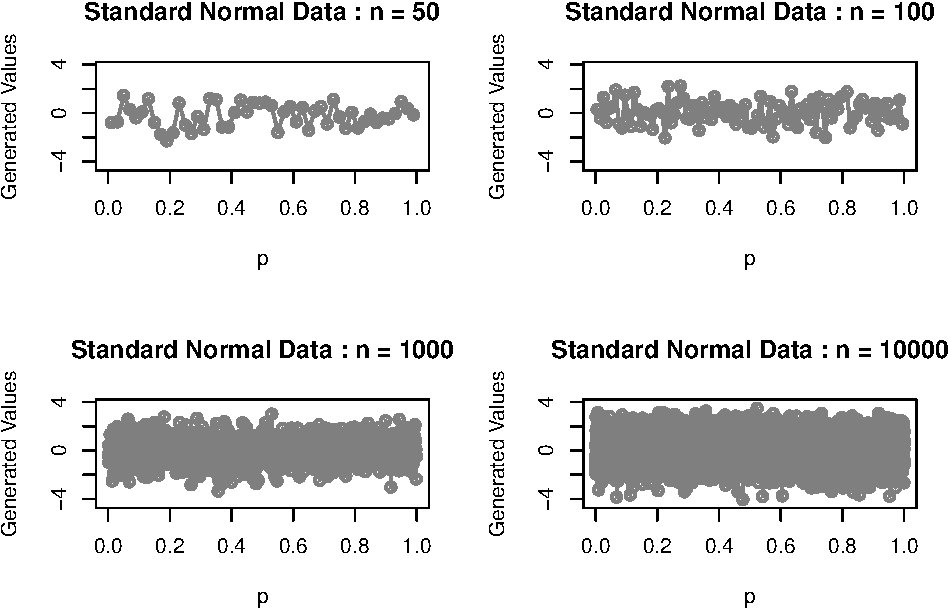
\includegraphics{a3_solutions_files/figure-latex/unnamed-chunk-7-1.pdf}

\begin{Shaded}
\begin{Highlighting}[]
\CommentTok{# student t(3) distribution array}
\KeywordTok{par}\NormalTok{(}\DataTypeTok{mfrow=}\KeywordTok{c}\NormalTok{(}\DecValTok{2}\NormalTok{,}\DecValTok{2}\NormalTok{))}

\ControlFlowTok{for}\NormalTok{(i }\ControlFlowTok{in} \DecValTok{1}\OperatorTok{:}\DecValTok{4}\NormalTok{) \{}
\NormalTok{  n =}\StringTok{ }\NormalTok{sample_sizes[i]}
\NormalTok{  p =}\StringTok{ }\KeywordTok{ppoints}\NormalTok{(n)}
\NormalTok{  title =}\StringTok{ "Student t(3) Data: n = "}
  
  \KeywordTok{plot}\NormalTok{(}\DataTypeTok{x =}\NormalTok{ p, }\DataTypeTok{y=}\NormalTok{data_t3[[i]], }
      \DataTypeTok{type=}\StringTok{"o"}\NormalTok{, }\DataTypeTok{lwd=}\DecValTok{2}\NormalTok{, }\DataTypeTok{col=}\StringTok{"grey50"}\NormalTok{,}
      \DataTypeTok{xlab=}\StringTok{"p"}\NormalTok{, }\DataTypeTok{ylab=}\StringTok{"Generated Values"}\NormalTok{,}
      \DataTypeTok{main=}\KeywordTok{paste0}\NormalTok{(title, n),}
      \DataTypeTok{xlim =}\KeywordTok{c}\NormalTok{(}\DecValTok{0}\NormalTok{,}\DecValTok{1}\NormalTok{), }\DataTypeTok{ylim =}\NormalTok{tlims)}
\NormalTok{\}}
\end{Highlighting}
\end{Shaded}

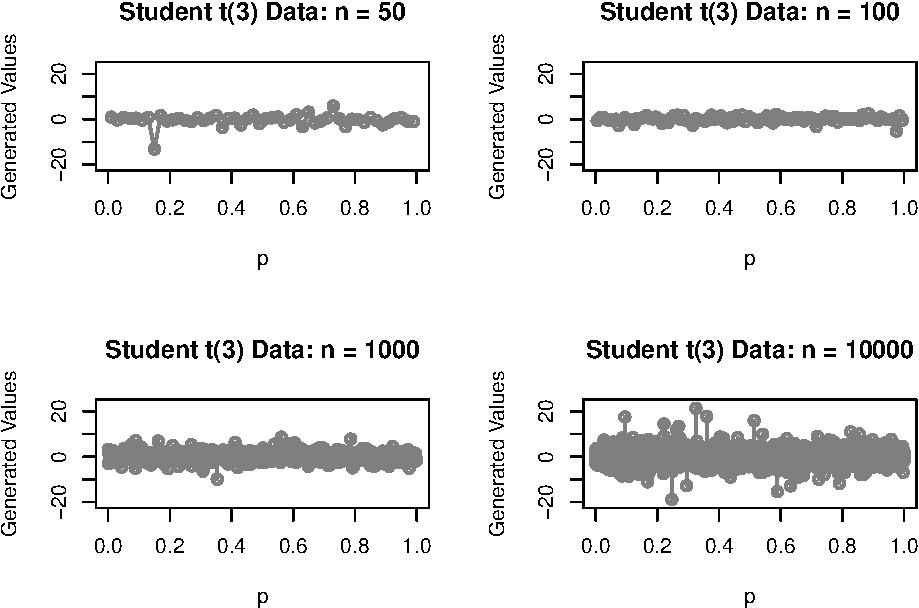
\includegraphics{a3_solutions_files/figure-latex/unnamed-chunk-7-2.pdf}

\begin{Shaded}
\begin{Highlighting}[]
\CommentTok{# Chi-Squared (3) distribution array}
\KeywordTok{par}\NormalTok{(}\DataTypeTok{mfrow=}\KeywordTok{c}\NormalTok{(}\DecValTok{2}\NormalTok{,}\DecValTok{2}\NormalTok{))}

\ControlFlowTok{for}\NormalTok{(i }\ControlFlowTok{in} \DecValTok{1}\OperatorTok{:}\DecValTok{4}\NormalTok{) \{}
\NormalTok{  n =}\StringTok{ }\NormalTok{sample_sizes[i]}
\NormalTok{  p =}\StringTok{ }\KeywordTok{ppoints}\NormalTok{(n)}
\NormalTok{  title =}\StringTok{ "Chi-Squared(3) Data : n = "}
  
  \KeywordTok{plot}\NormalTok{(}\DataTypeTok{x =}\NormalTok{ p, }\DataTypeTok{y=}\NormalTok{data_chi[[i]], }
      \DataTypeTok{type=}\StringTok{"o"}\NormalTok{, }\DataTypeTok{lwd=}\DecValTok{2}\NormalTok{, }\DataTypeTok{col=}\StringTok{"grey50"}\NormalTok{,}
      \DataTypeTok{xlab=}\StringTok{"p"}\NormalTok{, }\DataTypeTok{ylab=}\StringTok{"Generated Values"}\NormalTok{,}
      \DataTypeTok{main=}\KeywordTok{paste0}\NormalTok{(title, n),}
      \DataTypeTok{xlim =}\KeywordTok{c}\NormalTok{(}\DecValTok{0}\NormalTok{,}\DecValTok{1}\NormalTok{), }\DataTypeTok{ylim =}\NormalTok{clims)}
\NormalTok{\}}
\end{Highlighting}
\end{Shaded}

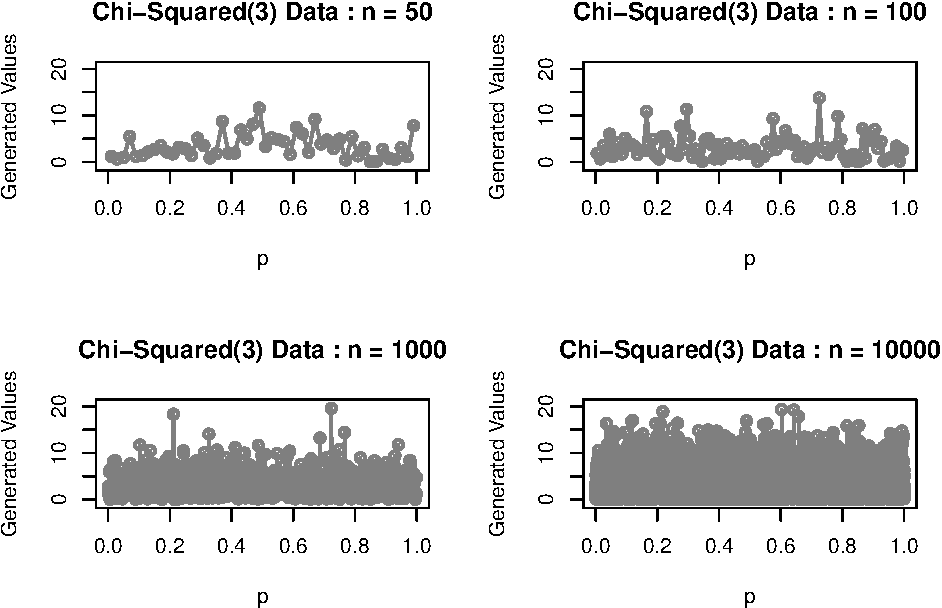
\includegraphics{a3_solutions_files/figure-latex/unnamed-chunk-7-3.pdf}

\item 

\textbf{(4 marks)} boxplots. Produce the three arrays of changing \(n\),
one for each distribution (\(N(0,1)\), \(t_3\), and \(\chi^2_3\)).
Submit each displayed array and comment on how the quality of the
display changes as \(n\) increases.

\begin{Shaded}
\begin{Highlighting}[]
\CommentTok{# normal distribution array}
\KeywordTok{par}\NormalTok{(}\DataTypeTok{mfrow=}\KeywordTok{c}\NormalTok{(}\DecValTok{2}\NormalTok{,}\DecValTok{2}\NormalTok{))}

\ControlFlowTok{for}\NormalTok{(i }\ControlFlowTok{in} \DecValTok{1}\OperatorTok{:}\DecValTok{4}\NormalTok{) \{}
\NormalTok{  n =}\StringTok{ }\NormalTok{sample_sizes[i]}
\NormalTok{  title =}\StringTok{ "Standard Normal Data : n = "}
  
  \KeywordTok{boxplot}\NormalTok{(}\DataTypeTok{x=}\NormalTok{data_norm[[i]], }\DataTypeTok{col=}\StringTok{"grey50"}\NormalTok{,}
      \DataTypeTok{ylab=}\StringTok{"Generated Values"}\NormalTok{,}
      \DataTypeTok{main=}\KeywordTok{paste0}\NormalTok{(title, n),}
      \DataTypeTok{ylim=}\NormalTok{zlims)}
\NormalTok{\}}
\end{Highlighting}
\end{Shaded}

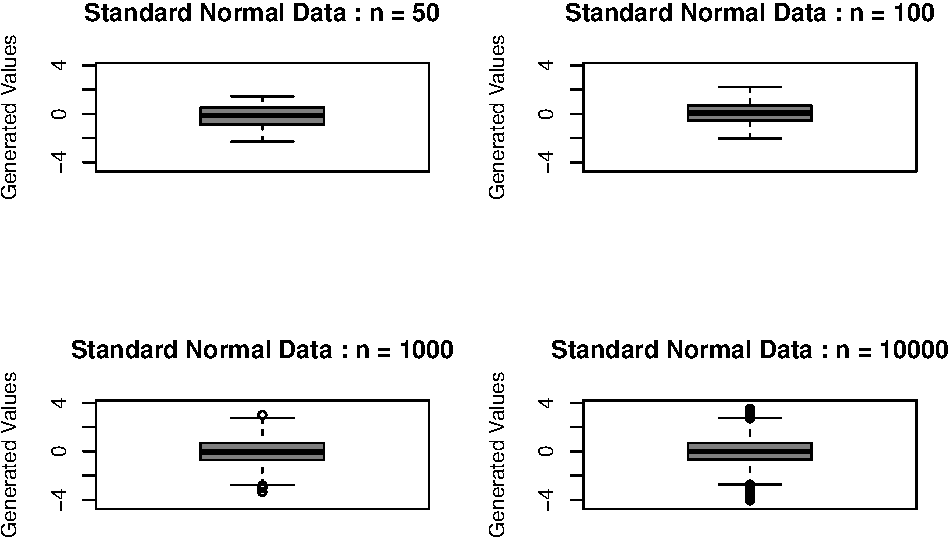
\includegraphics{a3_solutions_files/figure-latex/unnamed-chunk-8-1.pdf}

\begin{Shaded}
\begin{Highlighting}[]
\CommentTok{# student t(3) distribution array}
\KeywordTok{par}\NormalTok{(}\DataTypeTok{mfrow=}\KeywordTok{c}\NormalTok{(}\DecValTok{2}\NormalTok{,}\DecValTok{2}\NormalTok{))}

\ControlFlowTok{for}\NormalTok{(i }\ControlFlowTok{in} \DecValTok{1}\OperatorTok{:}\DecValTok{4}\NormalTok{) \{}
\NormalTok{  n =}\StringTok{ }\NormalTok{sample_sizes[i]}
\NormalTok{  title =}\StringTok{ "Student t(3) Data: n = "}
  
  \KeywordTok{boxplot}\NormalTok{(}\DataTypeTok{x=}\NormalTok{data_t3[[i]], }\DataTypeTok{col=}\StringTok{"grey50"}\NormalTok{,}
      \DataTypeTok{ylab=}\StringTok{"Generated Values"}\NormalTok{,}
      \DataTypeTok{main=}\KeywordTok{paste0}\NormalTok{(title, n),}
      \DataTypeTok{ylim=}\NormalTok{tlims)}
\NormalTok{\}}
\end{Highlighting}
\end{Shaded}

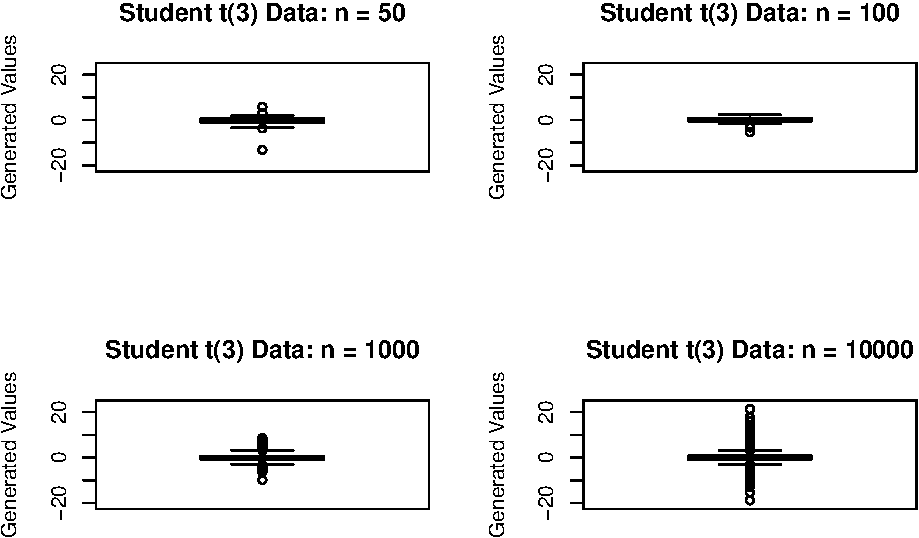
\includegraphics{a3_solutions_files/figure-latex/unnamed-chunk-8-2.pdf}

\begin{Shaded}
\begin{Highlighting}[]
\CommentTok{# Chi-Squared (3) distribution array}
\KeywordTok{par}\NormalTok{(}\DataTypeTok{mfrow=}\KeywordTok{c}\NormalTok{(}\DecValTok{2}\NormalTok{,}\DecValTok{2}\NormalTok{))}

\ControlFlowTok{for}\NormalTok{(i }\ControlFlowTok{in} \DecValTok{1}\OperatorTok{:}\DecValTok{4}\NormalTok{) \{}
\NormalTok{  n =}\StringTok{ }\NormalTok{sample_sizes[i]}
\NormalTok{  title =}\StringTok{ "Chi-Squared(3) Data : n = "}
  
  \KeywordTok{boxplot}\NormalTok{(}\DataTypeTok{x=}\NormalTok{data_chi[[i]], }\DataTypeTok{col=}\StringTok{"grey50"}\NormalTok{,}
      \DataTypeTok{ylab=}\StringTok{"Generated Values"}\NormalTok{,}
      \DataTypeTok{main=}\KeywordTok{paste0}\NormalTok{(title, n),}
      \DataTypeTok{ylim=}\NormalTok{clims)}
\NormalTok{\}}
\end{Highlighting}
\end{Shaded}

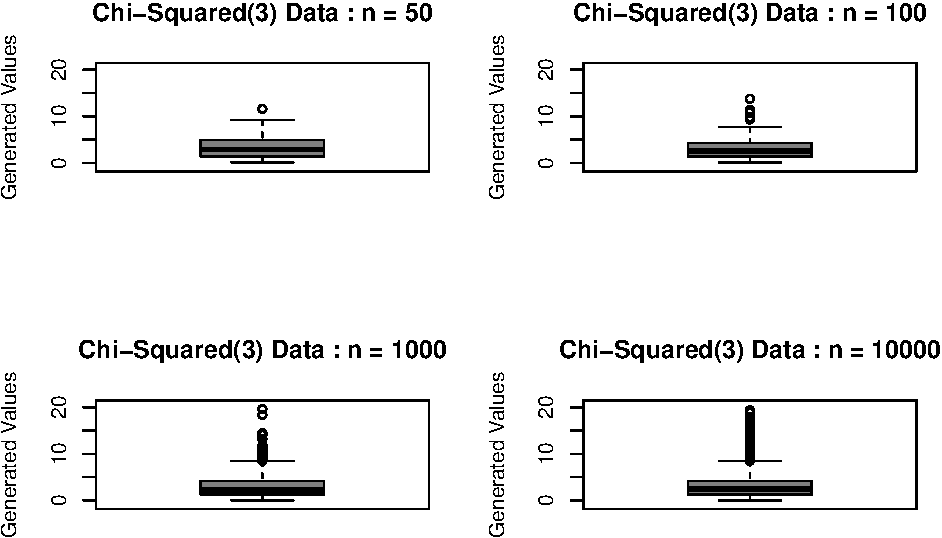
\includegraphics{a3_solutions_files/figure-latex/unnamed-chunk-8-3.pdf}

\item 

\textbf{(4 marks)} histograms Produce the three arrays of changing
\(n\), one for each distribution (\(N(0,1)\), \(t_3\), and
\(\chi^2_3\)). Submit each displayed array and comment on how the
quality of the display changes as \(n\) increases.

\item 

\textbf{(5 marks)} density plots Produce the three arrays of changing
\(n\), one for each distribution (\(N(0,1)\), \(t_3\), and
\(\chi^2_3\)). Submit each displayed array and comment on how the
quality of the display changes as \(n\) increases.

\begin{Shaded}
\begin{Highlighting}[]
\CommentTok{# normal distribution array}
\KeywordTok{par}\NormalTok{(}\DataTypeTok{mfrow=}\KeywordTok{c}\NormalTok{(}\DecValTok{2}\NormalTok{,}\DecValTok{2}\NormalTok{))}

\ControlFlowTok{for}\NormalTok{(i }\ControlFlowTok{in} \DecValTok{1}\OperatorTok{:}\DecValTok{4}\NormalTok{) \{}
\NormalTok{  n =}\StringTok{ }\NormalTok{sample_sizes[i]}
\NormalTok{  title =}\StringTok{ "Standard Normal Data : n = "}
\NormalTok{  dens =}\StringTok{ }\KeywordTok{density}\NormalTok{(data_norm[[i]], }\DataTypeTok{bw=}\StringTok{"SJ"}\NormalTok{, }\DataTypeTok{adjust =} \DecValTok{2}\NormalTok{)}
    
  \KeywordTok{plot}\NormalTok{(dens, }\DataTypeTok{col=}\StringTok{"grey50"}\NormalTok{, }
       \DataTypeTok{xlab=}\StringTok{"Generated Values"}\NormalTok{,}
       \DataTypeTok{main=}\KeywordTok{paste0}\NormalTok{(title, n),}
       \DataTypeTok{xlim=}\NormalTok{zlims, }\DataTypeTok{ylim=}\KeywordTok{c}\NormalTok{(}\DecValTok{0}\NormalTok{,}\FloatTok{0.5}\NormalTok{))}
  \KeywordTok{polygon}\NormalTok{(dens, }\DataTypeTok{col=}\StringTok{"grey50"}\NormalTok{)}
\NormalTok{\}}
\end{Highlighting}
\end{Shaded}

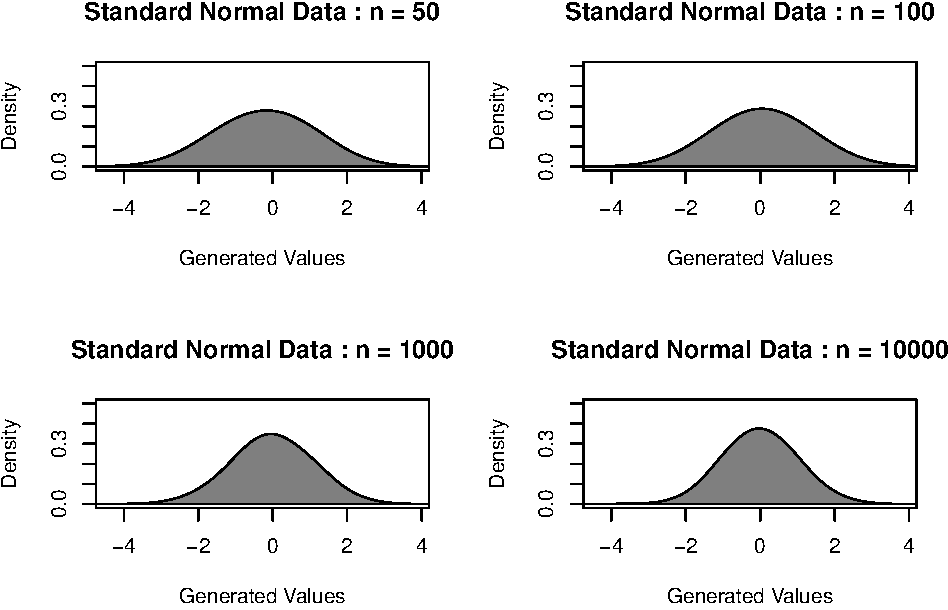
\includegraphics{a3_solutions_files/figure-latex/unnamed-chunk-9-1.pdf}

\begin{Shaded}
\begin{Highlighting}[]
\CommentTok{# student t(3) distribution array}
\KeywordTok{par}\NormalTok{(}\DataTypeTok{mfrow=}\KeywordTok{c}\NormalTok{(}\DecValTok{2}\NormalTok{,}\DecValTok{2}\NormalTok{))}

\ControlFlowTok{for}\NormalTok{(i }\ControlFlowTok{in} \DecValTok{1}\OperatorTok{:}\DecValTok{4}\NormalTok{) \{}
\NormalTok{  n =}\StringTok{ }\NormalTok{sample_sizes[i]}
\NormalTok{  title =}\StringTok{ "Student t(3) Data: n = "}
\NormalTok{  dens =}\StringTok{ }\KeywordTok{density}\NormalTok{(data_t3[[i]], }\DataTypeTok{bw=}\StringTok{"SJ"}\NormalTok{, }\DataTypeTok{adjust =} \DecValTok{2}\NormalTok{)}
    
  \KeywordTok{plot}\NormalTok{(dens, }\DataTypeTok{col=}\StringTok{"grey50"}\NormalTok{,}
       \DataTypeTok{xlab=}\StringTok{"Generated Values"}\NormalTok{,}
       \DataTypeTok{main=}\KeywordTok{paste0}\NormalTok{(title, n),}
       \DataTypeTok{xlim=}\NormalTok{tlims, }\DataTypeTok{ylim=}\KeywordTok{c}\NormalTok{(}\DecValTok{0}\NormalTok{,}\FloatTok{0.4}\NormalTok{))}
  \KeywordTok{polygon}\NormalTok{(dens, }\DataTypeTok{col=}\StringTok{"grey50"}\NormalTok{)}
\NormalTok{\}}
\end{Highlighting}
\end{Shaded}

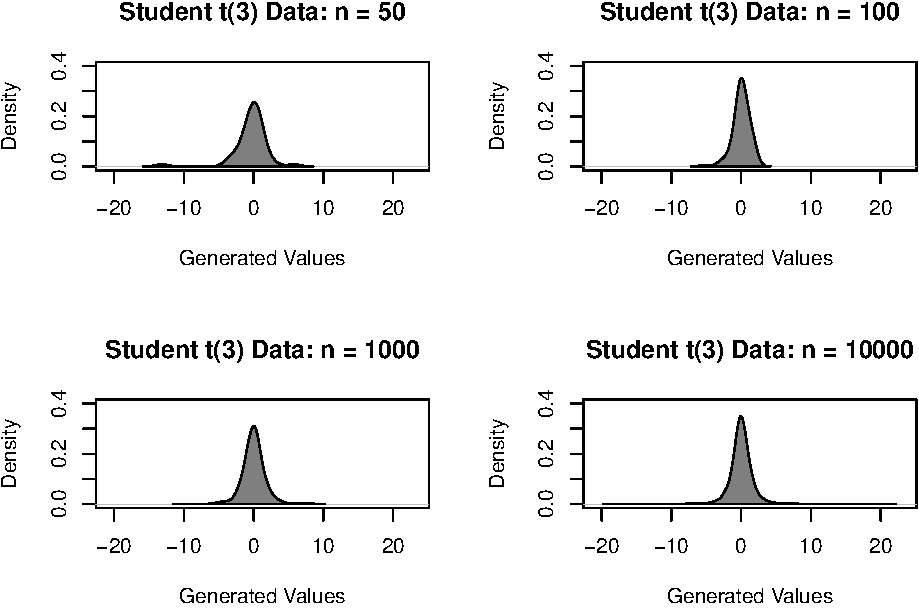
\includegraphics{a3_solutions_files/figure-latex/unnamed-chunk-9-2.pdf}

\begin{Shaded}
\begin{Highlighting}[]
\CommentTok{# Chi-Squared (3) distribution array}
\KeywordTok{par}\NormalTok{(}\DataTypeTok{mfrow=}\KeywordTok{c}\NormalTok{(}\DecValTok{2}\NormalTok{,}\DecValTok{2}\NormalTok{))}

\ControlFlowTok{for}\NormalTok{(i }\ControlFlowTok{in} \DecValTok{1}\OperatorTok{:}\DecValTok{4}\NormalTok{) \{}
\NormalTok{  n =}\StringTok{ }\NormalTok{sample_sizes[i]}
\NormalTok{  title =}\StringTok{ "Chi-Squared(3) Data : n = "}
\NormalTok{  dens =}\StringTok{ }\KeywordTok{density}\NormalTok{(data_chi[[i]], }\DataTypeTok{bw=}\StringTok{"SJ"}\NormalTok{, }\DataTypeTok{adjust =} \DecValTok{2}\NormalTok{)}
    
  \KeywordTok{plot}\NormalTok{(dens, }\DataTypeTok{col=}\StringTok{"grey50"}\NormalTok{, }
       \DataTypeTok{xlab=}\StringTok{"Generated Values"}\NormalTok{,}
       \DataTypeTok{main=}\KeywordTok{paste0}\NormalTok{(title, n),}
       \DataTypeTok{xlim=}\NormalTok{clims, }\DataTypeTok{ylim=}\KeywordTok{c}\NormalTok{(}\DecValTok{0}\NormalTok{,}\FloatTok{0.3}\NormalTok{))}
  \KeywordTok{polygon}\NormalTok{(dens, }\DataTypeTok{col=}\StringTok{"grey50"}\NormalTok{)}
\NormalTok{\}}
\end{Highlighting}
\end{Shaded}

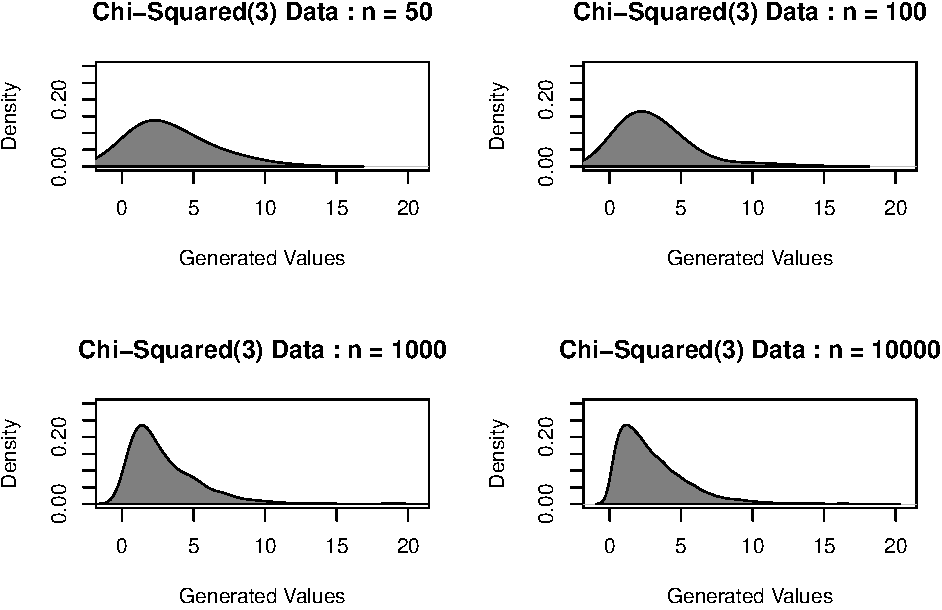
\includegraphics{a3_solutions_files/figure-latex/unnamed-chunk-9-3.pdf}

\eenum
\eenum

\item 

Have a look at the video \url{https://youtu.be/HEheh1BH34Q} which
compares the sizes of various astronomical bodies. The video tries to
give some sense of the comparative size of these bodies.

In the \texttt{R} code folder there is a file called \texttt{stars.R}
that contains measurements of the radius in kilometres of several
astronomical bodies in our solar system (in a vector called
\texttt{solarSystemRadii}) and of the radius of many stars as measured
in numbers of solar radii (in a vector called \texttt{starRadii}). Load
this file into \texttt{R} (use \texttt{source("directory/stars.R")} with
the \texttt{directory} changed to wherever you put the file
\texttt{stars.R}). For example:

\begin{Shaded}
\begin{Highlighting}[]
\KeywordTok{source}\NormalTok{(}\StringTok{"./stars.R"}\NormalTok{)}
\CommentTok{# Have a look at the contents of each}
\KeywordTok{head}\NormalTok{(solarSystemRadii)}
\end{Highlighting}
\end{Shaded}

\begin{verbatim}
##         radius
## Sun     696000
## Jupiter  69911
## Saturn   58232
## Uranus   25362
## Neptune  24622
## Earth     6371
\end{verbatim}

\begin{Shaded}
\begin{Highlighting}[]
\KeywordTok{head}\NormalTok{(starRadii)}
\end{Highlighting}
\end{Shaded}

\begin{verbatim}
##                    radius
## binarystarvvcephei   1900
## v354cephei           1520
## mucephei             1420
## kycygni              1420
## v509cassiopeiae       900
## v838monocerotis      1570
\end{verbatim}

\benum
\item In the video, the relative size of the planets is encoded in at
least three ways.

\benum
\item \textbf{(3 marks)} Name them.

Volume, position along a common scale, length

\item 

\textbf{(3 marks)} According to Stevens's law, which encoding is most
reliably encoded? Which least? (Justify your answers by appeal to this
law.)

According to Steven's law, length is most reliable encoding as it
creates the smallest bias when encoding the relative size of the
planets, which is due to its higher empirically observed range of values
\(0.9 \le \beta \le 1.1\), making \(p(x) \approx cx\). The least
reliable encoding is volume, which has the largest bias of the 3 when
encoding the relative size of the planets, due to its lower empirically
observed range of values \(0.5 \le \beta \le 0.8\).

\item 

\textbf{(1 marks)} How might position along a common scale have been
used instead? As the bodies being considered were all spheres, the
position along a common scale could have been used to display and
compare the radii (a measurement of length) of the bodies instead of the
volumes, which is only dependent on the radii and is a less accurate
encoding according to Steven's law.

\eenum

\item 

For the \texttt{solarSystemRadii} data:

Here you are going to draw the various astronomical bodies in our solar
system in much the same way as they appear in that video. You will be
making use of the \texttt{grid} package (as seen in previous
assignments).

You will need to recall a few things about \texttt{grid}. As before, you
will just be drawing circles to represent the various bodies so the
function \texttt{gridcircle(..)} will be used. Remember that (so far
anyway) that you are always drawing within a {[}0,1{]} rectangle do that
everything you draw will need to be translated to this range
(e.g.~dividing all radii by the maximum diameter will allow all circles
will fit within the unit square when centred at (0.5, 0.5).

You will also need a palette of colours, one for each body. How to
construct a palette of was described during an earlier lecture on
numbers and made available on the course web page.

The code below should give you some idea of what is possible. (See
help(\ldots{}) on any function to explore more parameter choices.)

\begin{Shaded}
\begin{Highlighting}[]
\KeywordTok{library}\NormalTok{(grid)}
\KeywordTok{library}\NormalTok{(colorspace)}
\NormalTok{cols <-}\StringTok{ }\KeywordTok{rainbow_hcl}\NormalTok{(}\DataTypeTok{n=}\DecValTok{5}\NormalTok{, }\DataTypeTok{c=}\DecValTok{100}\NormalTok{)  }\CommentTok{# 5 different colours having chroma = 100}

\KeywordTok{grid.newpage}\NormalTok{()}
\ControlFlowTok{for}\NormalTok{ (i }\ControlFlowTok{in} \DecValTok{1}\OperatorTok{:}\DecValTok{5}\NormalTok{) \{}
  \KeywordTok{grid.circle}\NormalTok{(}\DataTypeTok{x=}\FloatTok{0.5}\NormalTok{,}
              \DataTypeTok{y=}\FloatTok{0.5}\NormalTok{,}
              \DataTypeTok{r =}\NormalTok{ (}\DecValTok{6}\OperatorTok{-}\NormalTok{i)}\OperatorTok{/}\DecValTok{10}\NormalTok{,}
              \DataTypeTok{gp=}\KeywordTok{gpar}\NormalTok{(}\DataTypeTok{fill=}\KeywordTok{adjustcolor}\NormalTok{(cols[i], }\DataTypeTok{alpha.f =} \FloatTok{0.5}\NormalTok{))}
\NormalTok{  )}
\NormalTok{\}}
\CommentTok{# Now add a label and an arrow}
\NormalTok{xcentre <-}\StringTok{ }\FloatTok{0.5}
\NormalTok{ycentre <-}\StringTok{ }\FloatTok{0.5}
\NormalTok{degrees <-}\StringTok{ }\DecValTok{45}
\NormalTok{radians <-}\StringTok{ }\NormalTok{pi }\OperatorTok{*}\StringTok{ }\NormalTok{degrees }\OperatorTok{/}\StringTok{ }\DecValTok{180}
\NormalTok{arrowLength <-}\StringTok{ }\FloatTok{0.5} 
\NormalTok{xarrowFrom <-}\StringTok{ }\NormalTok{xcentre }\OperatorTok{+}\StringTok{ }\NormalTok{arrowLength }\OperatorTok{*}\StringTok{ }\KeywordTok{cos}\NormalTok{(radians)}
\NormalTok{yarrowFrom <-}\StringTok{ }\NormalTok{ycentre }\OperatorTok{+}\StringTok{ }\NormalTok{arrowLength }\OperatorTok{*}\StringTok{ }\KeywordTok{sin}\NormalTok{(radians)}
\NormalTok{xarrowTo <-}\StringTok{ }\NormalTok{xcentre }
\NormalTok{yarrowTo <-}\StringTok{ }\NormalTok{ycentre}
\CommentTok{# draw arrow}
\KeywordTok{grid.lines}\NormalTok{(}\DataTypeTok{x=}\KeywordTok{c}\NormalTok{(xarrowFrom, xarrowTo), }\DataTypeTok{y=}\KeywordTok{c}\NormalTok{(yarrowFrom, yarrowTo), }
           \DataTypeTok{arrow=}\KeywordTok{arrow}\NormalTok{(),}
           \DataTypeTok{gp =} \KeywordTok{gpar}\NormalTok{(}\DataTypeTok{col=}\StringTok{"black"}\NormalTok{, }\DataTypeTok{lwd=}\DecValTok{1}\NormalTok{, }\DataTypeTok{lty =} \DecValTok{1}\NormalTok{))}

\NormalTok{delta <-}\StringTok{ }\FloatTok{0.01}
\NormalTok{xText <-}\StringTok{ }\NormalTok{xarrowFrom }\OperatorTok{+}\StringTok{ }\NormalTok{delta }\OperatorTok{*}\StringTok{ }\KeywordTok{cos}\NormalTok{(radians)}
\NormalTok{yText <-}\StringTok{ }\NormalTok{yarrowFrom }\OperatorTok{+}\StringTok{ }\NormalTok{delta }\OperatorTok{*}\StringTok{ }\KeywordTok{sin}\NormalTok{(radians)}
\KeywordTok{grid.text}\NormalTok{(}\StringTok{"Centre"}\NormalTok{, }\DataTypeTok{x=}\NormalTok{ xText, }\DataTypeTok{y=}\NormalTok{ yText,}
          \DataTypeTok{just=}\StringTok{"left"}\NormalTok{, }\DataTypeTok{rot =}\NormalTok{ degrees,}
          \DataTypeTok{gp =} \KeywordTok{gpar}\NormalTok{(}\DataTypeTok{col=}\StringTok{"black"}\NormalTok{))}
\end{Highlighting}
\end{Shaded}

\begin{center}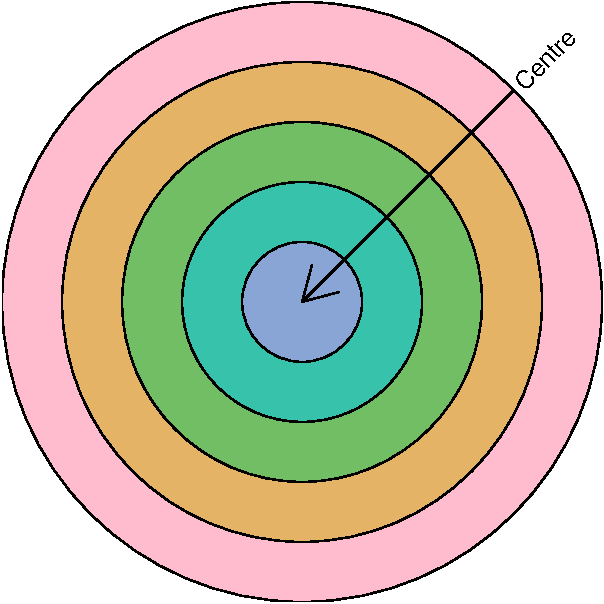
\includegraphics{a3_solutions_files/figure-latex/unnamed-chunk-11-1} \end{center}

These functions (and the \texttt{grid} package) are to be used to
address the following questions.

\benum
\item \textbf{(5 marks)} Represent each body by a circle whose radius is
proportional to the radius in kilometres of that body (use the radius of
the sun as the maximum possible radius in the display).

Align the circles so that they are all centred on (0.5, 0.5). Label each
of the three largest bodies (excluding the sun) on the plot. Show your
code and the picture produced.

\textbf{IMPORTANT:} you need to maintain an aspect ratio of 1 so begin
your \texttt{r} code chunks in \texttt{Rmarkdown} with something like
\texttt{\{r,\ fig.align="center",\ fig.width=4,\ fig.height=4\}}

\begin{Shaded}
\begin{Highlighting}[]
\KeywordTok{library}\NormalTok{(grid)}
\KeywordTok{library}\NormalTok{(colorspace)}

\NormalTok{xcentre =}\StringTok{ }\FloatTok{0.5}
\NormalTok{ycentre =}\StringTok{ }\FloatTok{0.5}
\NormalTok{cols =}\StringTok{ }\KeywordTok{rainbow_hcl}\NormalTok{(}\DecValTok{6}\NormalTok{, }\DataTypeTok{c =} \DecValTok{100}\NormalTok{)}
\NormalTok{n =}\StringTok{ }\KeywordTok{dim}\NormalTok{(solarSystemRadii)[}\DecValTok{1}\NormalTok{]}
\NormalTok{max_diam =}\StringTok{ }\NormalTok{solarSystemRadii[}\StringTok{'Sun'}\NormalTok{,]}
  
\KeywordTok{grid.newpage}\NormalTok{()}
\ControlFlowTok{for}\NormalTok{ (i }\ControlFlowTok{in} \DecValTok{1}\OperatorTok{:}\NormalTok{n) \{}
  \KeywordTok{grid.circle}\NormalTok{(}\DataTypeTok{x=}\NormalTok{xcentre,}
              \DataTypeTok{y=}\NormalTok{ycentre,}
              \DataTypeTok{r =}\NormalTok{ (solarSystemRadii[i,]}\OperatorTok{/}\NormalTok{max_diam)}\OperatorTok{/}\DecValTok{2}\NormalTok{,}
              \DataTypeTok{gp=}\KeywordTok{gpar}\NormalTok{(}\DataTypeTok{fill=}\KeywordTok{adjustcolor}\NormalTok{(cols[i], }\DataTypeTok{alpha.f =} \FloatTok{0.5}\NormalTok{))}
\NormalTok{  )}
\NormalTok{\}}

\NormalTok{degs =}\StringTok{ }\KeywordTok{c}\NormalTok{(}\DecValTok{45}\NormalTok{, }\DecValTok{135}\NormalTok{, }\DecValTok{315}\NormalTok{)}
\ControlFlowTok{for}\NormalTok{ (i }\ControlFlowTok{in} \DecValTok{2}\OperatorTok{:}\DecValTok{4}\NormalTok{) \{}
\NormalTok{  degrees =}\StringTok{ }\NormalTok{degs[i}\OperatorTok{-}\DecValTok{1}\NormalTok{]}
\NormalTok{  radians =}\StringTok{ }\NormalTok{pi }\OperatorTok{*}\StringTok{ }\NormalTok{degrees }\OperatorTok{/}\StringTok{ }\DecValTok{180}
\NormalTok{  arrowLength =}\StringTok{ }\FloatTok{0.5} 
\NormalTok{  xarrowFrom =}\StringTok{ }\NormalTok{xcentre }\OperatorTok{+}\StringTok{ }\NormalTok{arrowLength }\OperatorTok{*}\StringTok{ }\KeywordTok{cos}\NormalTok{(radians)}
\NormalTok{  yarrowFrom =}\StringTok{ }\NormalTok{ycentre }\OperatorTok{+}\StringTok{ }\NormalTok{arrowLength }\OperatorTok{*}\StringTok{ }\KeywordTok{sin}\NormalTok{(radians)}
  
  \ControlFlowTok{if}\NormalTok{ (degrees }\OperatorTok{==}\StringTok{ }\DecValTok{135}\NormalTok{) \{}
\NormalTok{    xarrowTo =}\StringTok{ }\NormalTok{xcentre }\OperatorTok{-}\StringTok{ }\NormalTok{(solarSystemRadii[i,]}\OperatorTok{/}\NormalTok{max_diam)}\OperatorTok{/}\DecValTok{2}
\NormalTok{  \} }\ControlFlowTok{else}\NormalTok{ \{}
\NormalTok{    xarrowTo =}\StringTok{ }\NormalTok{xcentre }\OperatorTok{+}\StringTok{ }\NormalTok{(solarSystemRadii[i,]}\OperatorTok{/}\NormalTok{max_diam)}\OperatorTok{/}\DecValTok{2}
\NormalTok{  \}}
  
\NormalTok{  yarrowTo =}\StringTok{ }\NormalTok{ycentre}
  \CommentTok{# draw arrow}
  \KeywordTok{grid.lines}\NormalTok{(}\DataTypeTok{x=}\KeywordTok{c}\NormalTok{(xarrowFrom, xarrowTo), }\DataTypeTok{y=}\KeywordTok{c}\NormalTok{(yarrowFrom, yarrowTo), }
             \DataTypeTok{arrow=}\KeywordTok{arrow}\NormalTok{(),}
             \DataTypeTok{gp =} \KeywordTok{gpar}\NormalTok{(}\DataTypeTok{col=}\StringTok{"black"}\NormalTok{, }\DataTypeTok{lwd=}\DecValTok{1}\NormalTok{, }\DataTypeTok{lty =} \DecValTok{1}\NormalTok{))}
  
\NormalTok{  delta =}\StringTok{ }\FloatTok{0.01}
\NormalTok{  xText =}\StringTok{ }\NormalTok{xarrowFrom }\OperatorTok{+}\StringTok{ }\NormalTok{delta }\OperatorTok{*}\StringTok{ }\KeywordTok{cos}\NormalTok{(radians)}
\NormalTok{  yText =}\StringTok{ }\NormalTok{yarrowFrom }\OperatorTok{+}\StringTok{ }\NormalTok{delta }\OperatorTok{*}\StringTok{ }\KeywordTok{sin}\NormalTok{(radians)}
  
\NormalTok{  body_name =}\StringTok{ }\KeywordTok{rownames}\NormalTok{(solarSystemRadii)[i]}
  \KeywordTok{grid.text}\NormalTok{(body_name, }\DataTypeTok{x=}\NormalTok{ xText, }\DataTypeTok{y=}\NormalTok{ yText,}
            \DataTypeTok{just=}\StringTok{"left"}\NormalTok{, }\DataTypeTok{rot =}\NormalTok{ degrees,}
            \DataTypeTok{gp =} \KeywordTok{gpar}\NormalTok{(}\DataTypeTok{col=}\StringTok{"black"}\NormalTok{))}
\NormalTok{\}}
\end{Highlighting}
\end{Shaded}

\begin{center}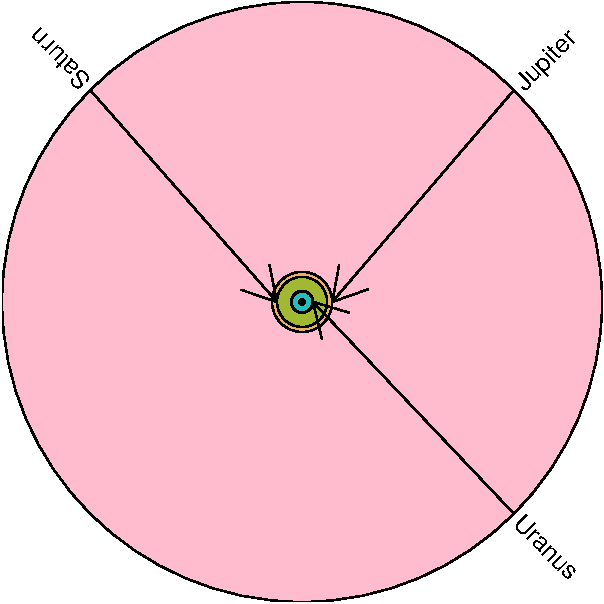
\includegraphics{a3_solutions_files/figure-latex/unnamed-chunk-12-1} \end{center}

\item 

\textbf{(2 marks)} Briefly comment on how easily it is to compare the
relative sizes of Uranus to Saturn? Of Saturn to Jupiter? Of Jupiter to
the Sun? How about comparing Uranus to the Earth or the Moon?

Because the two circles representing the planets are both relatively
large and are overlaid immediately (i.e.~with no other circle between
the two) over each other, and because the colors of the circles are
diverging, it is easy to see that Uranus is much smaller than Saturn as
we can still see much of the area of the circle representing Saturn.
However, it is difficult to determine by what proportion this difference
is as we comparing the two via their areas.

For Saturn and Jupiter, it is once again easy to compare the two planets
for the exact reasons mentioned above, with it being easy to determine
that Saturn is slightly larger than Jupiter. The same applies for
comparing Jupiter to the Sun, though it is harder to make this
comparison and most of Jupiter is not visible under the overlaying
circles.

Due to the Moon and Earth being significantly smaller than the Sun, they
are very difficult to see and compare with any of the other bodies. One
can tell that the Moon and Earth are smaller than Uranus, but it is
extremely difficult to determine the ratio of difference.

\item 

\textbf{(4 marks)} According to Stevens's law, what is the range of
values we might expect for the ratio of the areas (smaller to larger) of
each of the above comparisons? How do these compare to the ratio of
actual areas?

\[
\begin{array}{rll}
\text{Uranus vs. Saturn} &:& \displaystyle [(\frac{25362^2\pi}{58232^2\pi})^{0.9}, (\frac{25362^2\pi}{58232^2\pi})^{0.6}] = [0.2239955, 0.3688299]\\
\text{Saturn vs. Jupiter} &:& \displaystyle [(\frac{58232^2\pi}{69911^2\pi})^{0.9}, (\frac{58232^2\pi}{69911^2\pi})^{0.6}] = [0.7196298, 0.8030442]\\
\text{Jupiter vs. the Sun} &:& \displaystyle [(\frac{69911^2\pi}{696000^2\pi})^{0.9}, (\frac{69911^2\pi}{696000^2\pi})^{0.6}] = [0.01597663,0.06343421]\\
\text{Earth vs. Uranus} &:& \displaystyle [(\frac{6371^2\pi}{25362^2\pi})^{0.9}, (\frac{6371^2\pi}{25362^2\pi})^{0.6}] = [0.08318469, 0.1905588]\\
\text{The Moon vs. Uranus} &:& \displaystyle [(\frac{1737.1^2\pi}{25362^2\pi})^{0.9}, (\frac{1737.1^2\pi}{25362^2\pi})^{0.6}] = [0.00796984, 0.0398994]\\
\end{array}
\]

In comparison, the actual ratios are: \[
\begin{array}{rll}
\text{Uranus vs. Saturn} &:& 0.1896896\\
\text{Saturn vs. Jupiter} &:& 0.6937969\\
\text{Jupiter vs. the Sun} &:& 0.01008957\\
\text{Earth vs. Uranus} &:& 0.004691186\\
\text{The Moon vs. Uranus} &:& 0.06310274\\
\end{array}
\]

Every one of the ratio of actual areas falls outside and to the left of
the calculated ranges for the ratios. The demonstrates the bias and
reduced accuracy of using area as a visual encoding of magnititude.

\item 

\textbf{(5 marks)} Consider now all of the bodies in the solar system
\textbf{excluding the sun}. Using the \texttt{grid} package and
\texttt{grid.circle(...)} etc. lay out all of the remaining bodies from
the smallest at the left to the largest at the right with their centres
all at \(y=0.5\) but locate them so that they do not overlap. Have the
radius of each circles be proportional to the true radius of that body.
Mark the Earth, Uranus, Saturn, Jupiter on the plot.

Show your code and your output. Some functions you might find useful are
\texttt{order(...)} to determine the order of values and possibly
\texttt{\%in\%} as in \texttt{"foo"\ \%in\%\ c("foo",\ "bar")} will
return \texttt{TRUE} if the string \texttt{"foo"} can be found in the
vector \texttt{c("foo",\ "bar")}; the latter may be helpful in deciding
whether to label or not.

\begin{Shaded}
\begin{Highlighting}[]
\NormalTok{cols =}\StringTok{ }\KeywordTok{rainbow_hcl}\NormalTok{(n}\OperatorTok{-}\DecValTok{1}\NormalTok{)}

\NormalTok{asc_order =}\StringTok{ }\KeywordTok{order}\NormalTok{(solarSystemRadii)}
\NormalTok{planets =}\StringTok{ }\NormalTok{solarSystemRadii[asc_order[}\OperatorTok{!}\StringTok{ }\NormalTok{asc_order }\OperatorTok\StringTok{ }\KeywordTok{c}\NormalTok{(}\DecValTok{1}\NormalTok{)],]}
\NormalTok{planet_names =}\StringTok{ }\KeywordTok{rownames}\NormalTok{(solarSystemRadii)[asc_order[}\OperatorTok{!}\StringTok{ }\NormalTok{asc_order }\OperatorTok\StringTok{ }\KeywordTok{c}\NormalTok{(}\DecValTok{1}\NormalTok{)]]}
\NormalTok{total_length =}\StringTok{ }\DecValTok{2}\OperatorTok{*}\KeywordTok{sum}\NormalTok{(planets)}
\NormalTok{planetsr =}\StringTok{ }\NormalTok{planets}\OperatorTok{/}\NormalTok{total_length}

\NormalTok{xcenters =}\StringTok{ }\KeywordTok{replicate}\NormalTok{(n}\OperatorTok{-}\DecValTok{1}\NormalTok{, }\DecValTok{0}\NormalTok{)}
\ControlFlowTok{for}\NormalTok{ (i }\ControlFlowTok{in} \DecValTok{1}\OperatorTok{:}\NormalTok{(n}\OperatorTok{-}\DecValTok{1}\NormalTok{)) \{}
\NormalTok{  xcenters[i] =}\StringTok{ }\NormalTok{(}\DecValTok{2}\OperatorTok{*}\KeywordTok{sum}\NormalTok{(planetsr[}\DecValTok{1}\OperatorTok{:}\NormalTok{i}\OperatorTok{-}\DecValTok{1}\NormalTok{])) }\OperatorTok{+}\StringTok{ }\NormalTok{planetsr[i]}
\NormalTok{\}}

\KeywordTok{grid.newpage}\NormalTok{()}
\NormalTok{xcenter =}\StringTok{ }\DecValTok{0}
\NormalTok{ycenter =}\StringTok{ }\FloatTok{0.5}

\ControlFlowTok{for}\NormalTok{ (i }\ControlFlowTok{in} \DecValTok{1}\OperatorTok{:}\NormalTok{(n}\OperatorTok{-}\DecValTok{1}\NormalTok{)) \{}
  \KeywordTok{grid.circle}\NormalTok{(}\DataTypeTok{x=}\NormalTok{xcenters[i],}
              \DataTypeTok{y=}\NormalTok{ycenter,}
              \DataTypeTok{r =}\NormalTok{ planetsr[i],}
              \DataTypeTok{gp=}\KeywordTok{gpar}\NormalTok{(}\DataTypeTok{fill=}\KeywordTok{adjustcolor}\NormalTok{(cols[i], }\DataTypeTok{alpha.f =} \FloatTok{0.5}\NormalTok{)))}
  
\NormalTok{  body_name =}\StringTok{ }\NormalTok{planet_names[i]}
  \ControlFlowTok{if}\NormalTok{ (body_name }\OperatorTok\StringTok{ }\KeywordTok{c}\NormalTok{(}\StringTok{'Earth'}\NormalTok{, }\StringTok{'Uranus'}\NormalTok{, }\StringTok{'Saturn'}\NormalTok{, }\StringTok{'Jupiter'}\NormalTok{)) \{}
    \KeywordTok{grid.text}\NormalTok{(body_name, }\DataTypeTok{x=}\NormalTok{xcenters[i], }\DataTypeTok{y=}\FloatTok{0.09}\NormalTok{,}
              \DataTypeTok{just=}\StringTok{"left"}\NormalTok{,}
              \DataTypeTok{gp =} \KeywordTok{gpar}\NormalTok{(}\DataTypeTok{col=}\StringTok{"black"}\NormalTok{))}
\NormalTok{  \}}
\NormalTok{\}}
\end{Highlighting}
\end{Shaded}

\begin{center}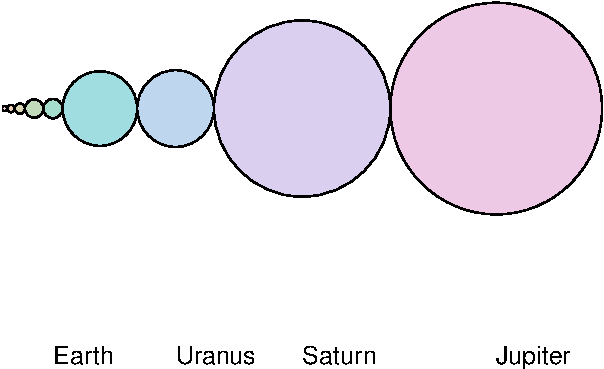
\includegraphics{a3_solutions_files/figure-latex/unnamed-chunk-13-1} \end{center}

\eenum      

\item 

For the \texttt{stars} data, \benum
\item \textbf{(3 marks)} Construct a quantile plot of the radii of the
\texttt{stars}. Describe whatever patterns you see in the data.

\begin{Shaded}
\begin{Highlighting}[]
\NormalTok{n =}\StringTok{ }\KeywordTok{dim}\NormalTok{(starRadii)[}\DecValTok{1}\NormalTok{]}
\NormalTok{p =}\StringTok{ }\KeywordTok{ppoints}\NormalTok{(n)}
\NormalTok{starRadii =}\StringTok{ }\NormalTok{starRadii[}\KeywordTok{order}\NormalTok{(starRadii),]}
\KeywordTok{plot}\NormalTok{(}\DataTypeTok{x =}\NormalTok{ p, }\DataTypeTok{y=}\NormalTok{starRadii, }
      \DataTypeTok{type=}\StringTok{"o"}\NormalTok{, }\DataTypeTok{lwd=}\DecValTok{2}\NormalTok{, }\DataTypeTok{col=}\StringTok{"grey50"}\NormalTok{,}
      \DataTypeTok{xlab=}\StringTok{"p"}\NormalTok{, }\DataTypeTok{ylab=}\StringTok{"Radius"}\NormalTok{,}
      \DataTypeTok{main=}\StringTok{"Quantile Plot of Stars' Radii"}\NormalTok{,}
      \DataTypeTok{xlim =}\KeywordTok{c}\NormalTok{(}\DecValTok{0}\NormalTok{,}\DecValTok{1}\NormalTok{))}
\end{Highlighting}
\end{Shaded}

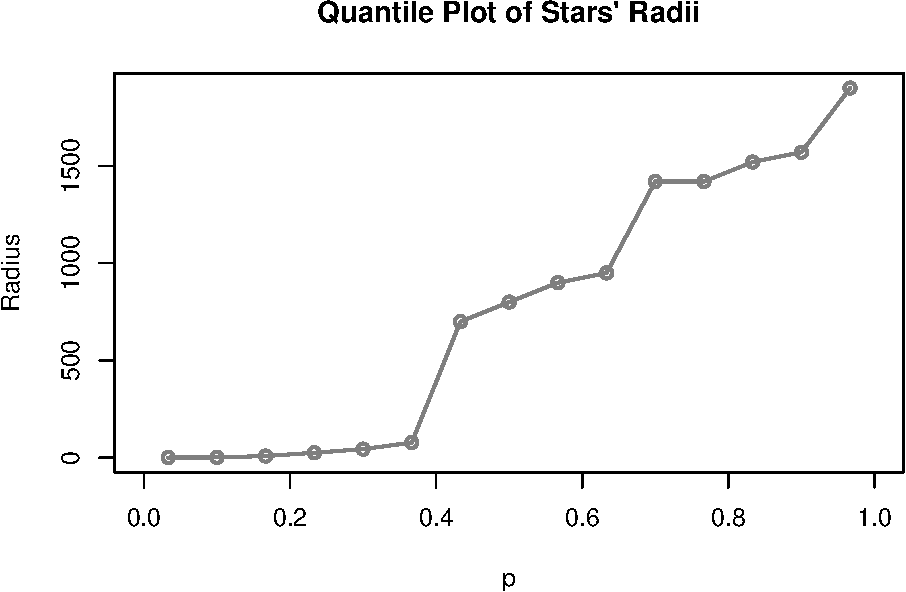
\includegraphics{a3_solutions_files/figure-latex/unnamed-chunk-14-1.pdf}

The data appears to be somewhat discrete with the main values being at
\(0\), \(\sim700-1000\), \(1500\).

\item 

\textbf{(3 marks)} Construct a quantile plot of the volume of the
\texttt{stars}. (Recall: the volume of a sphere is
\(\frac{4}{3}\pi r^3\).) Describe whatever patterns you see in the data.

\begin{Shaded}
\begin{Highlighting}[]
\NormalTok{starVolumes =}\StringTok{ }\DecValTok{4}\OperatorTok{*}\NormalTok{(starRadii}\OperatorTok{^}\DecValTok{3}\NormalTok{)}\OperatorTok{/}\DecValTok{3}
\KeywordTok{plot}\NormalTok{(}\DataTypeTok{x =}\NormalTok{ p, }\DataTypeTok{y=}\NormalTok{starVolumes, }
      \DataTypeTok{type=}\StringTok{"o"}\NormalTok{, }\DataTypeTok{lwd=}\DecValTok{2}\NormalTok{, }\DataTypeTok{col=}\StringTok{"grey50"}\NormalTok{,}
      \DataTypeTok{xlab=}\StringTok{"p"}\NormalTok{, }\DataTypeTok{ylab=}\StringTok{"Volume"}\NormalTok{,}
      \DataTypeTok{main=}\StringTok{"Quantile Plot of Stars' Volumes"}\NormalTok{,}
      \DataTypeTok{xlim =}\KeywordTok{c}\NormalTok{(}\DecValTok{0}\NormalTok{,}\DecValTok{1}\NormalTok{))}
\end{Highlighting}
\end{Shaded}

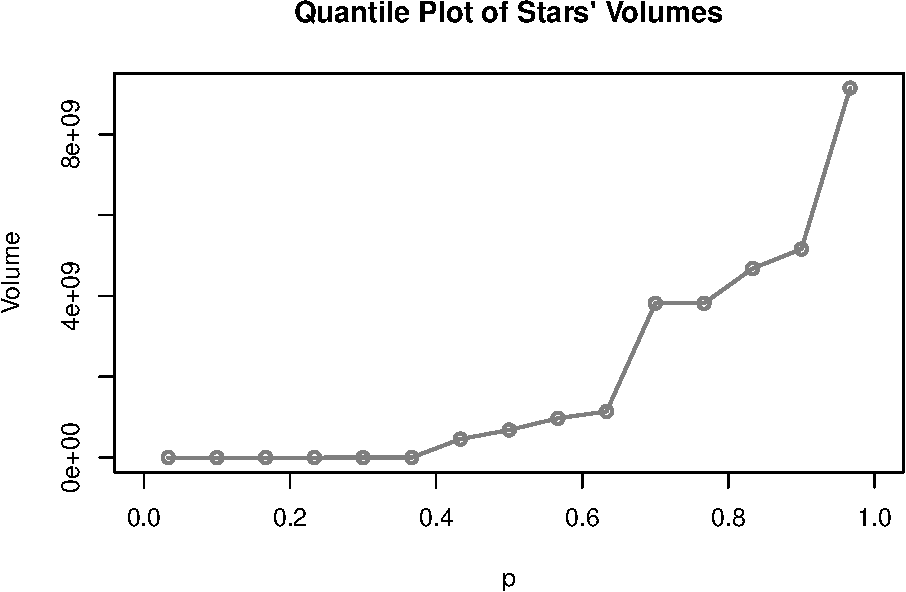
\includegraphics{a3_solutions_files/figure-latex/unnamed-chunk-15-1.pdf}

\item 

\textbf{(2 marks)} How do these two summaries differ?

The plots have similar shapes, but

\item 

\textbf{(3 marks)} Construct a quantile plot of the base 10 logarithms
of the stellar radii. Describe whatever patterns you see in the data.

\begin{Shaded}
\begin{Highlighting}[]
\NormalTok{starLogs =}\StringTok{ }\KeywordTok{log}\NormalTok{(starRadii, }\DataTypeTok{base=}\DecValTok{10}\NormalTok{)}
\KeywordTok{plot}\NormalTok{(}\DataTypeTok{x =}\NormalTok{ p, }\DataTypeTok{y=}\NormalTok{starLogs, }
      \DataTypeTok{type=}\StringTok{"o"}\NormalTok{, }\DataTypeTok{lwd=}\DecValTok{2}\NormalTok{, }\DataTypeTok{col=}\StringTok{"grey50"}\NormalTok{,}
      \DataTypeTok{xlab=}\StringTok{"p"}\NormalTok{, }\DataTypeTok{ylab=}\StringTok{"Volume"}\NormalTok{,}
      \DataTypeTok{main=}\StringTok{"Quantile Plot of Stars' Base-10 Logarithms"}\NormalTok{,}
      \DataTypeTok{xlim =}\KeywordTok{c}\NormalTok{(}\DecValTok{0}\NormalTok{,}\DecValTok{1}\NormalTok{))}
\end{Highlighting}
\end{Shaded}

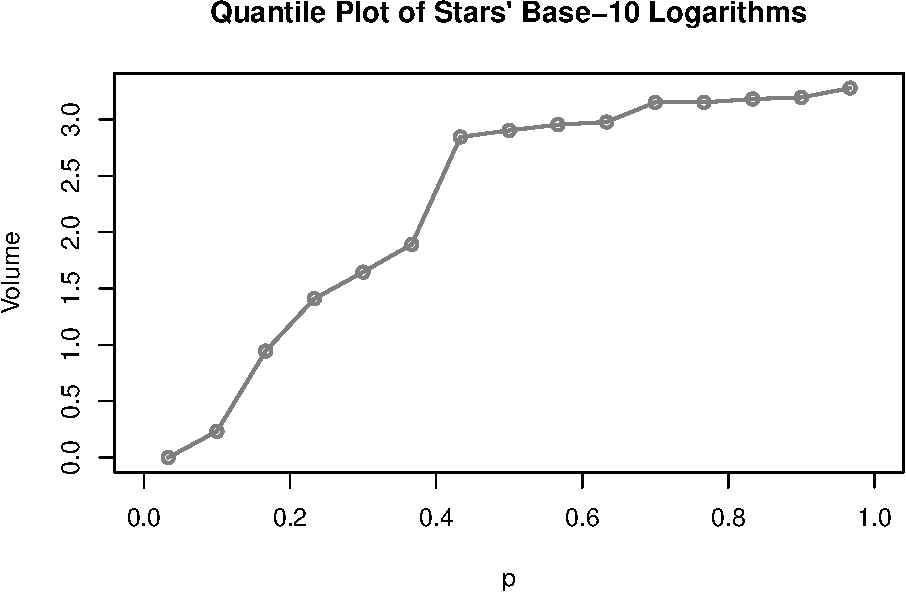
\includegraphics{a3_solutions_files/figure-latex/unnamed-chunk-16-1.pdf}

The data seems to have a decreasing cumulative distribution function as
\(Q(p)\) and \(p\) have an inverse relationship. There is a sharp drop
in \(Q(p)\) at \(p \approx 0.55\).

\item 

\textbf{(4 marks)} Again construct a quantile plot of the logarithms of
the stellar radii \textbf{but} this time use base 2 logarithms. In the
same plot, overlay the quantiles for the base 10 logarithms. Explain how
and why the two sets of quantiles differ.

\begin{Shaded}
\begin{Highlighting}[]
\NormalTok{starLog2s =}\StringTok{ }\KeywordTok{log}\NormalTok{(starRadii, }\DataTypeTok{base=}\DecValTok{2}\NormalTok{)}
\NormalTok{ylims =}\StringTok{ }\KeywordTok{extendrange}\NormalTok{(}\KeywordTok{c}\NormalTok{(starLogs, starLog2s))}

\KeywordTok{plot}\NormalTok{(}\DataTypeTok{x =}\NormalTok{ p, }\DataTypeTok{y=}\NormalTok{starLogs, }
      \DataTypeTok{type=}\StringTok{"o"}\NormalTok{, }\DataTypeTok{lwd=}\DecValTok{2}\NormalTok{, }\DataTypeTok{col=}\StringTok{"red"}\NormalTok{,}
      \DataTypeTok{xlab=}\StringTok{"p"}\NormalTok{, }\DataTypeTok{ylab=}\StringTok{"Volume"}\NormalTok{,}
      \DataTypeTok{main=}\StringTok{"Quantile Plot of Stars' Logarithms"}\NormalTok{,}
      \DataTypeTok{xlim =}\KeywordTok{c}\NormalTok{(}\DecValTok{0}\NormalTok{,}\DecValTok{1}\NormalTok{), }\DataTypeTok{ylim=}\NormalTok{ylims)}

\KeywordTok{par}\NormalTok{(}\DataTypeTok{new =} \OtherTok{TRUE}\NormalTok{)}

\KeywordTok{plot}\NormalTok{(}\DataTypeTok{x =}\NormalTok{ p, }\DataTypeTok{y=}\NormalTok{starLog2s, }
      \DataTypeTok{type=}\StringTok{"o"}\NormalTok{, }\DataTypeTok{lwd=}\DecValTok{2}\NormalTok{, }\DataTypeTok{col=}\StringTok{"blue"}\NormalTok{,}
      \DataTypeTok{ylab=}\StringTok{"Volume"}\NormalTok{,}
      \DataTypeTok{xlim =}\KeywordTok{c}\NormalTok{(}\DecValTok{0}\NormalTok{,}\DecValTok{1}\NormalTok{), }\DataTypeTok{ylim=}\NormalTok{ylims)}
\end{Highlighting}
\end{Shaded}

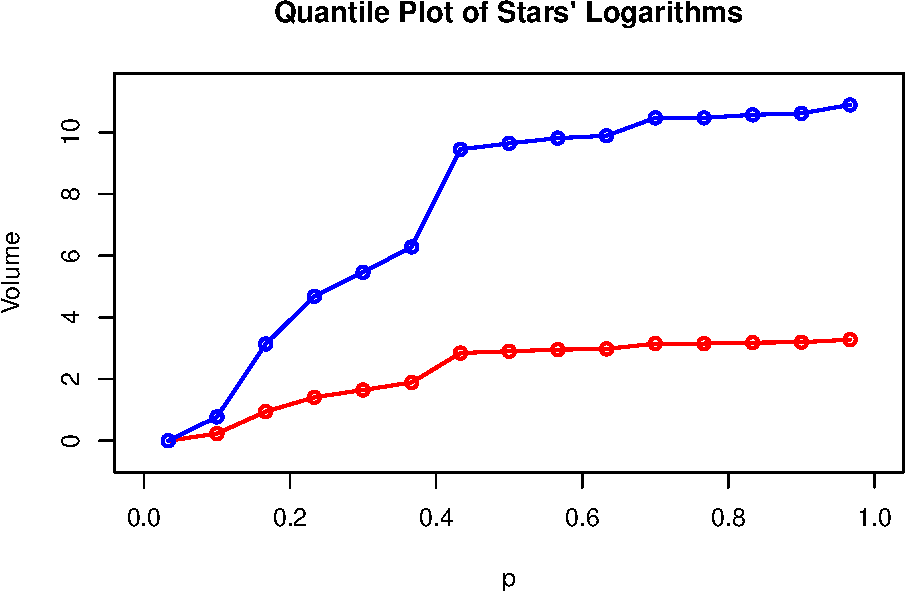
\includegraphics{a3_solutions_files/figure-latex/unnamed-chunk-17-1.pdf}

\eenum
\eenum
\eenum


\end{document}
